\documentclass[tikz]{standalone}

\usetikzlibrary{intersections,decorations.markings}

\tikzset{
  % arrowhead marking which way a contour is traversed
  flow/.style={decoration={markings, mark=at position #1 with {\arrow[ultra thick]{>}}},
    postaction={decorate}},
  flow/.default=0.15,
  zcontour/.style={circle, minimum width=4cm},
  wdisk/.style={circle, minimum width=1.2cm},
}
% dots at the origin and at the pole w
\newcommand{\poles}[2]{%
  \filldraw (#1) circle (2pt) node [above right] {0} (#2) circle (2pt) node [right]{$w$};}
% angle from the center of node #2 to node #3, stored in the macro #1
\newcommand{\angleto}[3]{%
  \pgfmathanglebetweenpoints{\pgfpointanchor{#2}{center}}{\pgfpointanchor{#3}{center}}%
  \let#1\pgfmathresult}

\begin{document}

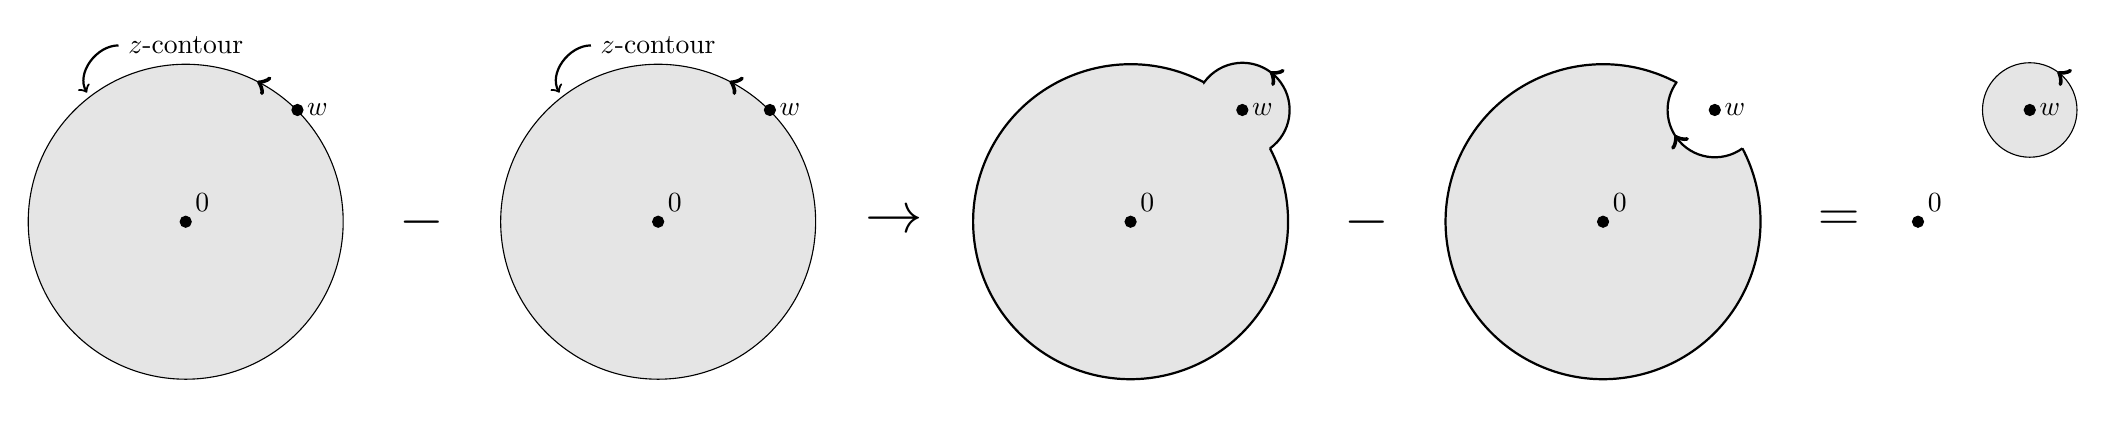
\begin{tikzpicture}

  \node [zcontour, fill=gray!20, draw=black, name path=A, flow=0.175] at (0,0) (A) {};
  \node [wdisk, name path=C] at (A.north east) (B) {};
  \poles{A}{B}
  \node [above] at (A.north) (annotation) {$z$-contour};
  \draw [thick] (annotation.west) edge[out=180,in=120,->] ++(-0.4,-0.6);

  \node [zcontour, fill=gray!20, draw=black, name path=C, flow=0.175] at (6cm,0) (C) {};
  \node [wdisk, name path=D] at (C.north east) (D) {};
  \poles{C}{D}
  \node [above] at (C.north) (annotation) {$z$-contour};
  \draw [thick] (annotation.west) edge[out=180,in=120,->] ++(-0.4,-0.6);

  \node [zcontour, fill=gray!20, name path=E] at (12cm,0) (E) {};
  \node [wdisk, fill=gray!20, name path=F, flow] at (E.north east) (F) {};
  \poles{E}{F}

  % intersection points between circles E and F
  \path [name intersections={of = E and F}];
  \coordinate (EF1) at (intersection-1);
  \coordinate (EF2) at (intersection-2);

  % angles from the centers of E and F to their intersection points
  \angleto{\EEFone}{E}{EF1}
  \angleto{\EEFtwo}{E}{EF2}
  \angleto{\FEFone}{F}{EF1}
  \angleto{\FEFtwo}{F}{EF2}

  % draw outline
  \draw[thick]
  (EF2) arc[start angle=\FEFtwo-360, end angle=\FEFone,radius=0.6cm] --
  (EF1) arc[start angle=\EEFone-360, end angle=\EEFtwo,radius=2cm];

  \node [zcontour, fill=gray!20, name path=G] at (18cm,0) (G) {};
  \node [wdisk, fill=white, name path=H] at (G.north east) (H) {};
  \poles{G}{H}

  % intersection points between circles G and H
  \path [name intersections={of = G and H}];
  \coordinate (GH1) at (intersection-1);
  \coordinate (GH2) at (intersection-2);

  % draw outline
  \draw[thick, flow=0.075]
  (GH2) arc[start angle=\FEFtwo-360, end angle=\FEFone-360,radius=0.6cm] --
  (GH1) arc[start angle=\EEFone-360, end angle=\EEFtwo,radius=2cm];

  \node [zcontour] at (22cm,0) (E) {};
  \node [wdisk, draw=black, fill=gray!20, flow] at (E.north east) (F) {};
  \poles{E}{F}

  {\huge
  \draw (3cm,0) node {$-$} (9cm,0) node {$\to$} (15cm,0) node {$-$} (21cm,0) node {$=$};
  }

\end{tikzpicture}

\end{document}
